\section{Question 1}
\subsection{part a.}

\begin{figure}[H]
	\centering
  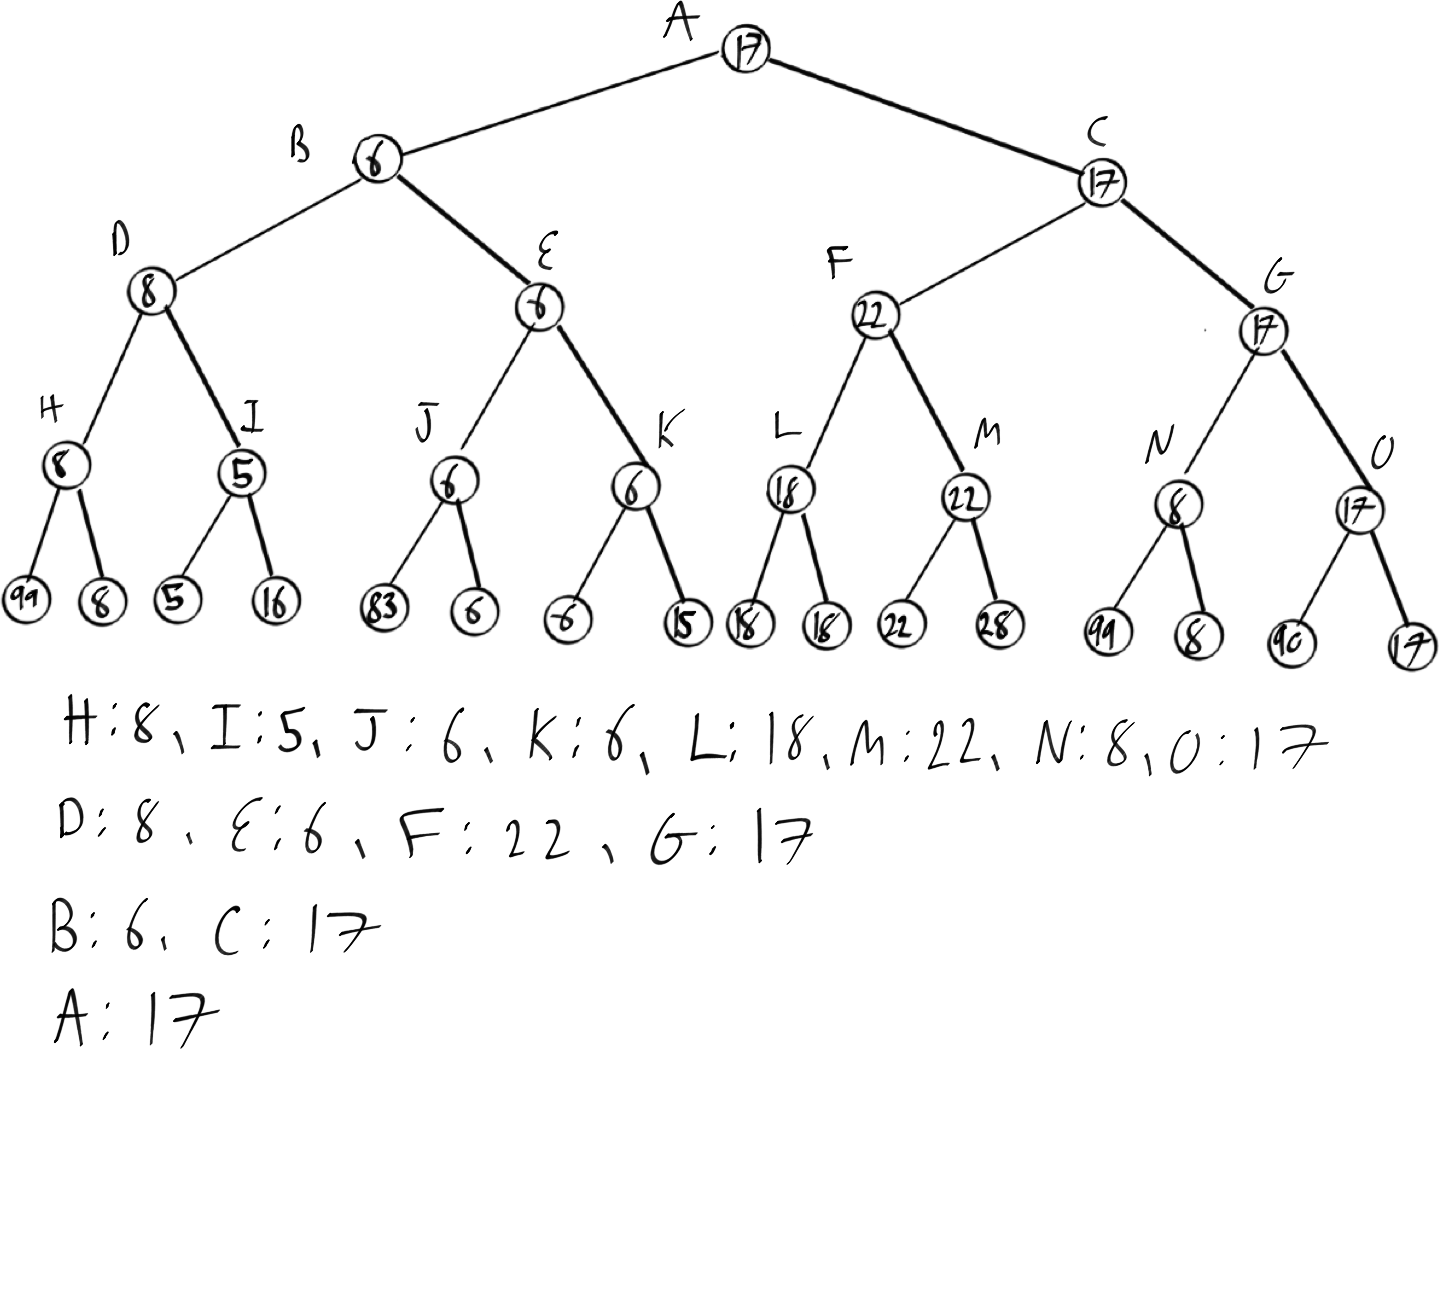
\includegraphics[scale = 0.65]{q1_part_a.png}
	\caption{Question 1: Part a}
	\label{fig: Q1 Part a}
\end{figure}


\subsection{part b.}

\begin{figure}[H]
	\centering
  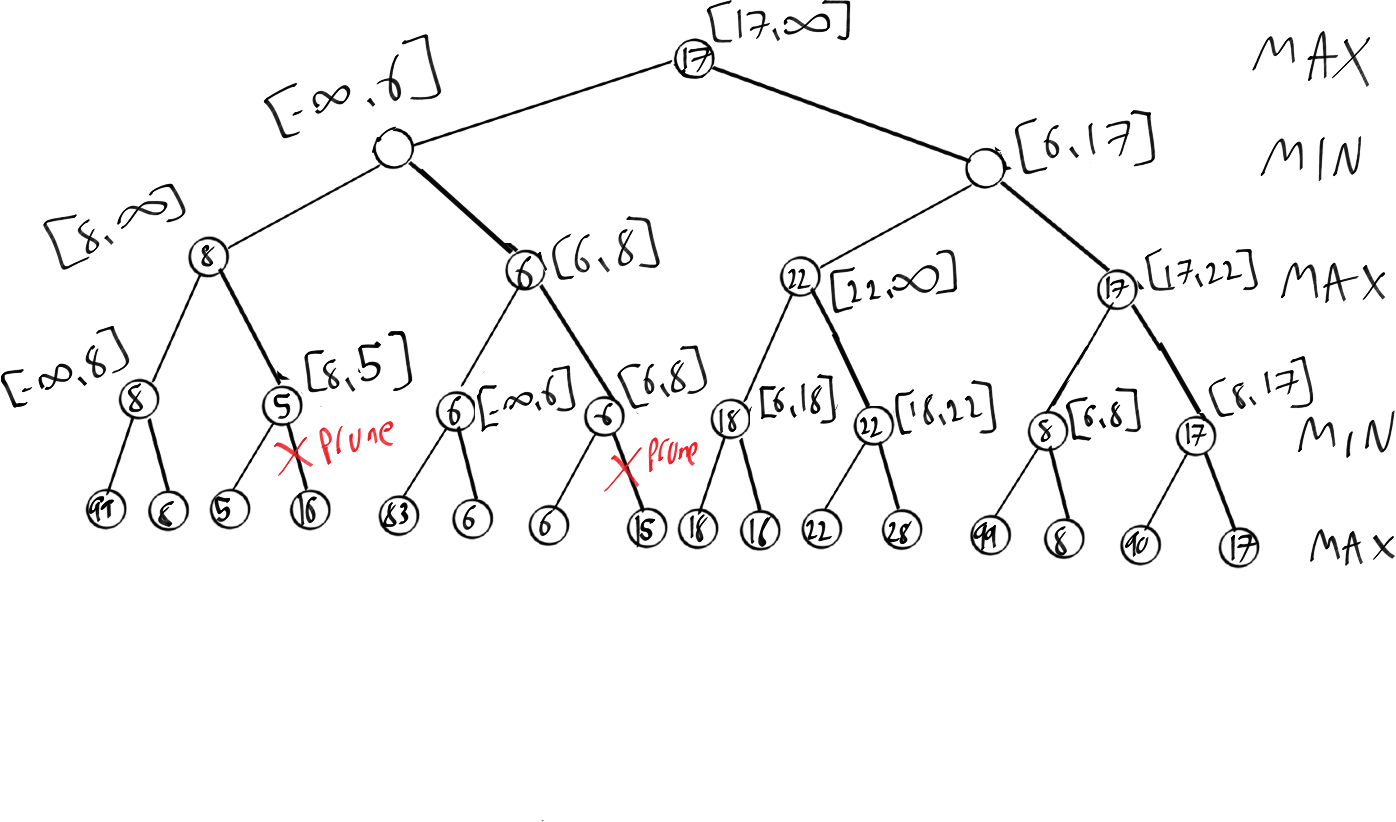
\includegraphics[scale = 0.65]{q1_part_b.png}
	\caption{Question 1: Part b}
	\label{fig: Q1 Part b}
\end{figure}


\subsection{part c.}
The diagrams for parts a. and b. both show that the exhaustive minimax algorithm,
and the minimax algorithm with alpha-beta pruning reach the same Max value for the
root node: 17. This is not a coincidence and should happen in the general case, as
alpha-beta pruning is simply meant to disregard the nodes that will not be worth considering. However,
the underlying assumption is the opponent is playing optimally. If the opponent is playing suboptimal, the results of
the minimax and alpha-beta pruning are not necessarily the best.

\subsection{part d.}

\begin{figure}[H]
	\centering
  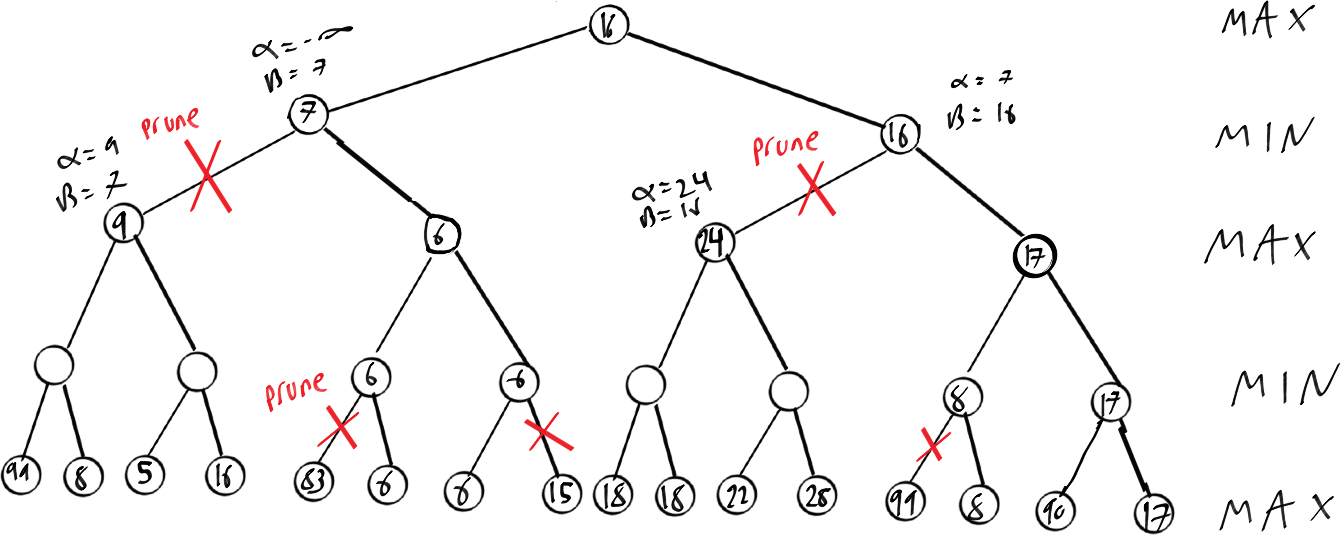
\includegraphics[scale = 0.65]{q1_part_d.png}
	\caption{Question 1: Part d}
	\label{fig: Q1 Part d}
\end{figure}

First the minimax algorithm is run at nodes B,C,D,E backs up the value 7 to node b, and the value 16 to node c.

When the alpha beta pruning algorithm is ran

depth 1: alpha = - inf, beta = 7
depth 2: alpha = 9, beta = 7 [Prune Sub tree]

The left child of node b is pruned, and alpha beta continues down to depth 4.

depth 2: alpha = 7, beta = 7
depth 3: alpha = 7, beta = 7
depth 4: alpha = 83, beta = 6 [Prune]
depth 4: alpha = 6, beta = 7

This will back up 6 to node J, the alpha beta pruning will now go to the right child of
node b.

depth 3: alpha = 7, beta = 7
depth 4: alpha = 6, beta = 7
This will back up 6 to node K

The value 15 is pruned since its greater than the value backed up at its parent.

The left traversal of the alpha-beta pruning is done, now it starts doing right traversal.

Nodes Examined:
Nodes Not Examined: 14

Similarly, to the left side alpha beta pruning cuts off node e

\subsection{part e.}

\begin{figure}[H]
	\centering
  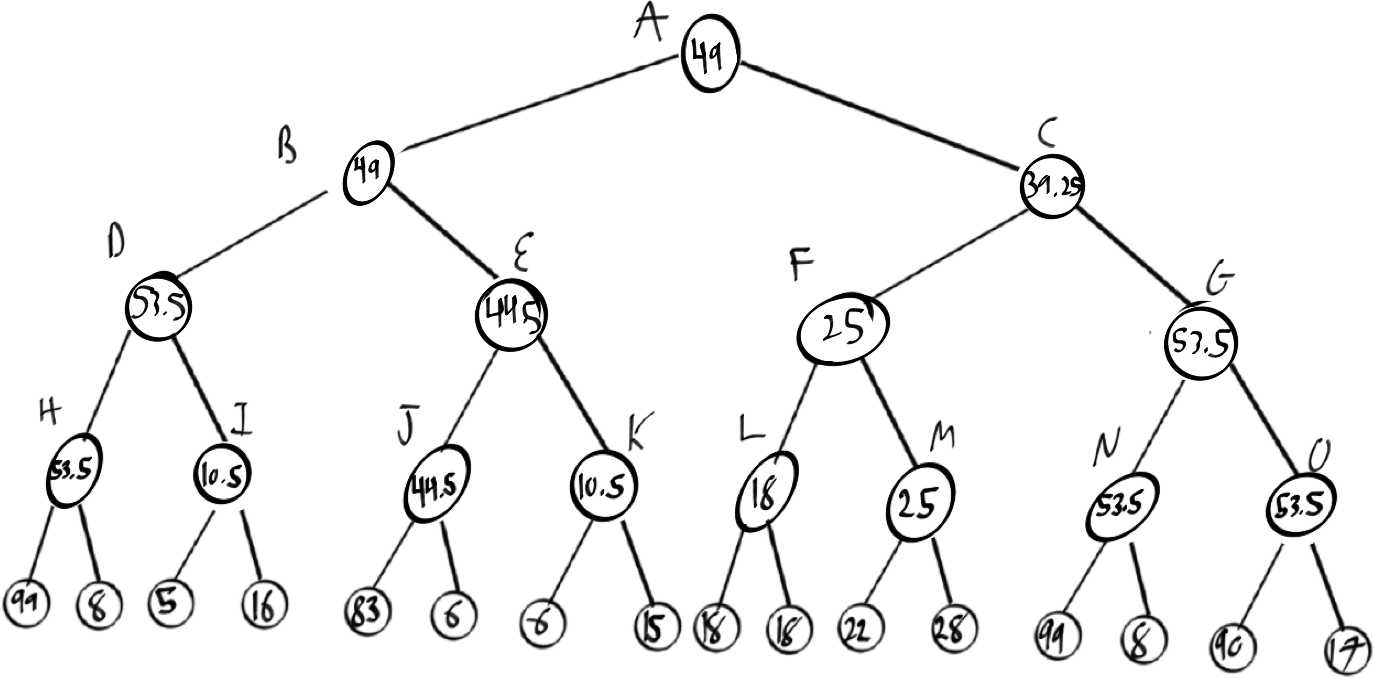
\includegraphics[scale = 0.65]{q1_part_e.png}
	\caption{Question 1: Part e}
	\label{fig: Q1 Part e}
\end{figure}

Applying the minimax algorithm using expected values...

\begin{center}
Expected Values of Nodes H,I,J,K,L,N,N,O... \\
Node H: 0.5 * (99 + 8)  = 53.5 \tab \tab
Node I: 0.5 * (5 + 16)  = 10.5 \\
Node J: 0.5 * (83 + 6)  = 44.5 \tab \tab
Node K: 0.5 * (6 + 15)  = 10.5 \\
Node L: 0.5 * (18 + 18) = 18   \tab \tab
Node M: 0.5 * (22 + 28) = 25   \\
Node N: 0.5 * (99 + 8)  = 53.5 \tab \tab
Node O: 0.5 * (90 + 17) = 53.5 \\

\newpage
Nodes D, E, F, G choose the Max \\
Node D: 53.5 \tab \tab
Node E: 44.5 \\
Node F: 25   \tab \tab
Node G: 53.5 \\

Expected values of Nodes B, C \\
Node B: 0.5 * (53.5 + 44.5) = 49 \tab \tab
Node C: 0.5 * (25 + 53.5)   = 39.25

Node A: 49
\end{center}

The root node value has a value of 49, which is the expected value for the scenario of the opponent
choosing a random node.

We can apply alpha beta pruning algorithm, although first the minimax algorithm will need to find the expected values at each of the nodes. Using the algorithm after this step
begs the question of why should we use the alpha beta pruning algorithm in the first place. If we use all of the computational resources to calculate those expected values then
using the alpha beta pruning algorithm is redundant and doesn't provide any utility.

This shows that alpha beta pruning may not be the most efficient algorithm in the case of a suboptimal opponent, as there are better choices to choose from.


\subsection{NOTCOMPLETE}
NOT DONE: CAN WE APPLY ALPHA BETA PRUNING IN THIS CASE
